% !TEX root = paper.tex

\section{Introduction}

The CP decomposition is a low-rank approximation of a multi-dimensional array, or tensor, which generalizes matrix approximations like the truncated singular value decomposition. As in Figure \ref{fig:cpdecomposition}, CP decomposition approximates the given input matrix as sum of $k$ rank-1 tensors.  CP is often used for finding hidden patterns, or latent factors, within tensor data, particularly when the goal is to interpret the factors, and it is popular within the signal processing, machine learning, and scientific computing communities.

\begin{figure}[htbp]
\begin{center}
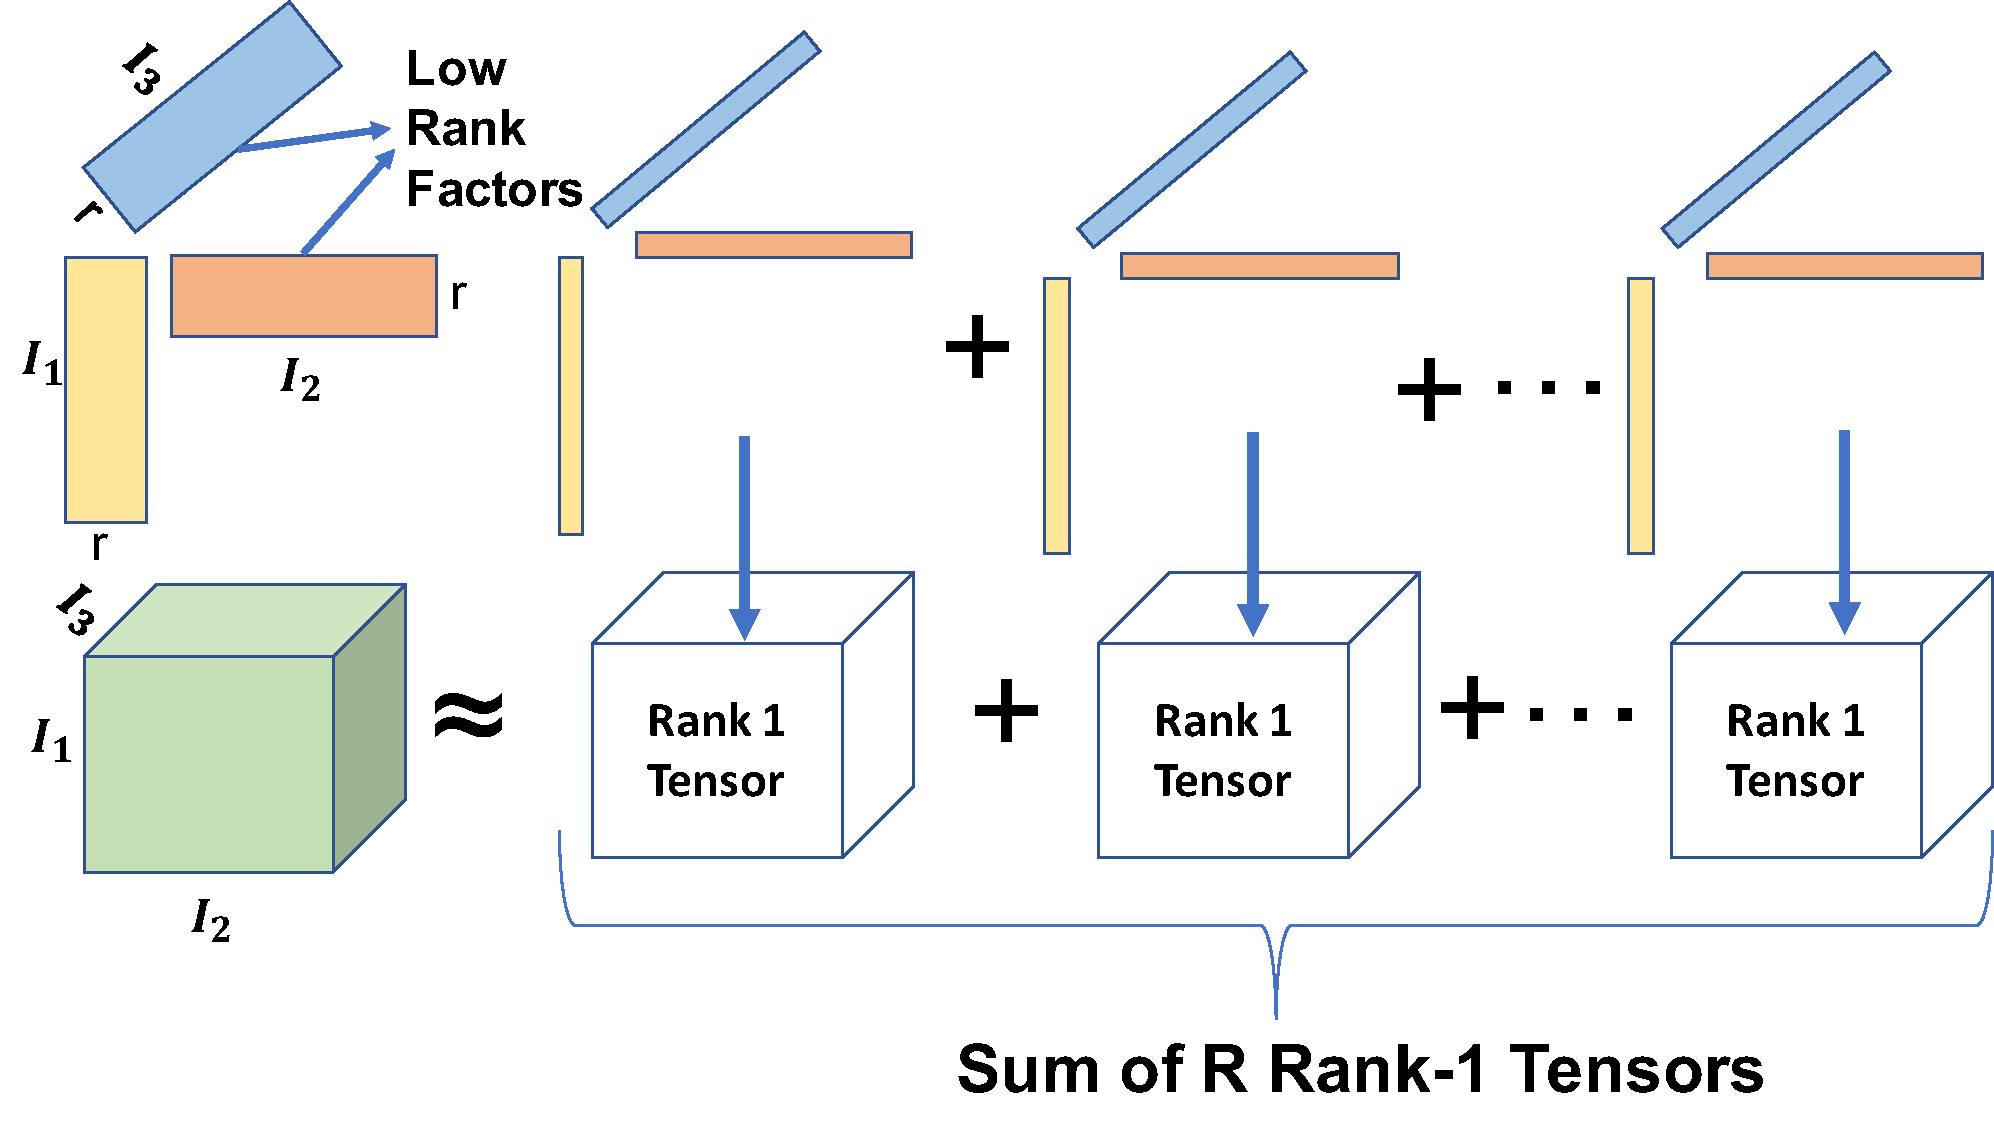
\includegraphics[width=3in, height=1.5in]{fig/cpdecomposition.pdf}
\caption{CP Decomposition}
\label{fig:cpdecomposition}
\end{center}
\end{figure}


To aid in interpretability, domain-specific constraints are often imposed on the computed factors.
We focus in this paper on dense tensors (when nearly all of the tensor entries are nonzero) and on constraining solutions to have nonnegative entries, which is useful when the tensor data itself is nonnegative. Formally, NNCP can be defined as
\SplitN{\label{eqn:nncp}}{
\min_{\HH^{(i)} \geq 0} & \| \TA - \CP \|_F^2 \\ 
\min_{\HH^{(i)} \geq 0} & \| \TA - \sum_{r=1}^R \Mn{H}{1}(:,r) \circ \cdots \circ \Mn{H}{N}(:,r) \|_F^2
}
where $\|\M{X}\|_F=(\sum_{ij} x_{ij}^2)^{1/2}$ is the Frobenius norm.

For example, in imaging and microscopy applications, tensor values often correspond to intensities, and NNCP can be used to cluster and analyze the data in a lower-dimensional space \cite{JC+16}.
In this work, we consider two such applications: a series of time-lapse hyperspectral images \cite{FAN16} and a dynamic functional correlation data set generated from functional magnetic resonance images of human brains \cite{VEU+12}.

One approach to handling multidimensional data is to ``matricize'' it, combining sets of modes to reshape the data into a matrix, so that standard matrix  methods like principal component analysis or nonnegative matrix factorization can be applied.
While this approach can be effective in certain cases, reshaping the data destroys multidimensional relationships among entries that the matrix methods cannot recover.
By maintaining the tensor structure of the data, the low-rank representations preserve these relationships, often producing better and more interpretable results.

However, tensor methods are more complicated both mathematically and computationally.
The kernel computations within standard algorithms for computing NNCP can be formulated as matrix computations, but the complicated layout of tensors in memory prevents the straightforward use of BLAS and LAPACK libraries.
In particular, the matrix formulation of subcomputations involve different views of the tensor data, so no single layout yields a column- or row-major matrix layout for all subcomputations.
Likewise, the parallelization approach for tensor methods is not a straightforward application of parallel matrix computation algorithms.

In developing an efficient parallel algorithm for computing a NNCP of a dense tensor, the key is to parallelize the bottleneck computation known as Matricized-Tensor Times Khatri-Rao Product (MTTKRP), which is performed repeatedly for each mode of the tensor.
The parallelization must load balance the computation, minimize communication across processors, and distribute the results so that the rest of the computation can be performed independently.
In our algorithm, not only do we load balance the computation, but we also compute and store temporary values that can be used across MTTKRPs of different modes using a technique known as dimension trees, significantly reducing the computational cost compared to standard approaches.
Our parallelization strategy also avoids communicating tensor entries and minimizes the communication of factor matrix entries, helping the algorithm to remain computation bound and scalable to high core counts.

As we detail in the related work, the general techniques for reducing computation and communication are not new.
The recomputation avoidance was proposed in a sequential algorithm \cite{PTC13a}, and the parallelization scheme was proposed and analyzed for general tensors \cite{BKR17-TR} and the algorithm was implemented for 3D tensors \cite{LK+17b}.
The main contribution of this paper is the combination and implementation of these ideas for general $N$D tensors, and we demonstrate superior performance to the existing implementation for 3D tensors \cite{LK+17b}.

We summarize our main contributions as follows:
\begin{itemize}
		\item we present a computation- and communication-efficient algorithm for NNCP with detailed cost analysis,
		\item our algorithm is designed for general $N$-way tensors,
		\item we demonstrate a performance improvement of up to \grey{$2.2\times$} over the existing state-of-the-art parallel software on 3D tensors,
		\item we demonstrate efficient parallel scaling of up to \grey{$253\times$} on \grey{$512$} cores.
\end{itemize}